\documentclass{article}

\usepackage[utf8]{inputenc}
\usepackage{ngerman}

\usepackage{graphicx}
\usepackage{subfigure}
\usepackage{float}

\usepackage{lipsum}
\usepackage{pdfpages}

\usepackage{varioref}
	\labelformat{figure}{Abbildung~#1}


\begin{document}
%opening

\includepdf{Titlepage}

\newpage

\tableofcontents

\newpage
	
\section{Einleitung}


Das Technical Design Document stellt die technischen und strukturellen Anforderung an unser
Spiel dar. Zuerst gehen wir auf unsere Coding Conventions ein. Danach geben wir eine Auflistung
unserer verwendeten Tools, die für die Entwicklung des Spiels benötigt werden. Des Weiteren
gehen wir auf die Struktur des Spiels ein durch Klassen- und Use Case Diagramme. Zum Schluss
gibt dieses Dokument Auskunft über die Projektplanung mit ihren Arbeitspaketen und
Meilensteinen.

\vspace{2cm}

\subsection{Das Projekt}


Veil of Death ist ein Level basierter Runner in dem der Spieler versucht mit dem Protagonisten aus einer Festung zu entkommen und entsprechenden Hindernissen auszuweichen ohne in den ihn verfolgenden Nebel zu geraten. Rennen tut der Protagonist selbstständig. Der Spieler muss den Hindernissen durch Springen, Rutschen und dadurch, dass er die Lane wechselt ausweichen.
Man bekommt einen Score und eine Wertung am Ende jeden Levels, welche einem sagt, wie gut
man abgeschnitten hat. Sollte der Spieler sterben muss er das jeweilige Level von vorne beginnen.

\newpage

\section{Programmierung}

\vspace{1cm}

\subsection{Programmiersprache}

Die Programmiersprache für die wir uns entschieden haben ist C\#. Einerseits erleichtert die Ähnlichkeit zu Java, die Arbeit im Team, da
jeder im Team bereits Erfahrungen in der Programmierung mit Java gesammelt hat. Weiterhin wird C\# uns als Programmiersprache von
dem Monogame Framework vorgeschrieben.

\vspace{1cm}

\subsection{Coding Conventions}


Format-Vorgaben \newline
• je Zeile nur 1 Anweisung (" '\{" ' und " '\}" ' zählen jeweils als eine Anweisung; " 'else" ' ist eine
anweisung, danach immer enter) \newline
• wenn eine Klammerung \{\} länger als 10 Zeilen ist, wird die schließende Klammer
kommentiert (z.B: " '\} // end if(true)" ' , " '\} //end class(player)); das erleichtert die Lesbarkeit
um einiges.\newline
• zugehörige Codefragmente sind durch Einrücken deutlich zu machen (z.B.: nach
" 'if(bedingung)" ' oder " 'else" ' ist in der nächsten Zeile ein zu rücken, gilt rekursiv ->
Mehrfachverschachtelung)\newline
\newline
Klassen-Variablen\newline
1-2 stelliges kleingeschriebenes Präfix zur Typbezeichnung + " '\_" ' vor dem Variablennamen in
CamelCase groß beginnend.\newline
• t\_VariablenName (Time)\newline
• sp\_VariablenName (Sprite)\newline
• tx\_VariablenName (Textur)\newline
• m\_VariablenName (Model)\newline
• O\_VariablenName (GameObject)\newline
• x\_VariablenName (Matrix)\newline
• peVariablenName (PanelElement -Sprite)\newline
• ptVariablenName (PanelElement -Text)\newline
\newline

\noindent Standard-Variablen\newline
Einstelliges klein geschriebenes Präfix zur Typbezeichnung + Variablennamen in CamelCase groß
beginnend.\newline
• iVariablenName (integer)\newline
• fVariablenName (float)\newline
• sVariablenName (String)\newline
\newline
Jede Variabel vom Typ Bool ist immer mit Frage-Präfix zu Bennenen
Bsp.: bool isCollactable, hasLoot, isActive, canRespawn;\newline
Kommentieren\newline
• Kommentare, die Funktionen und Methoden dokumentieren sind mit " 'summary" '
einzupflegen\newline
• übergebene Parameter sind mit " 'param" ' zu erklären\newline
• Summary wird in in Visual Studio mit 3 /// eingeleitet (Macro)\newline
• Beispiel:\newline
/// $<$summary$>$\newline
/// kurze sinnvolle Beschreibung.\newline
/// $<$/summary$>$\newline
/// $<$param name=" '\_uebergabeParameter" '$>$ Was soll übergeben werden $<$/param$>$
private void doStuff(var \_uebergabeParameter) \{...\}\newline


\subsection{Verwendete Tools}

• Blender\newline
Für die Modellierung des Charakters und der Gegner wird Blender verwendet.
Die fertigen Modelle werden als .fbx exportiert um dann mit Monogame importiert zu
werden. Alle Modelle im .stl Format werden importiert und zu .fbx konvertiert.\newline
• Solid Edge\newline
Für die Modellierung von Hindernissen und dem Rest der Spielwelt sowie
Collectables wird Solid Edge verwendet. Die Dateien werden als .stl exportiert um
dann mit Blender konvertiert zu werden.\newline
• Audacity\newline
Mit Audacity werden die entsprechenden Soundeffekte und auch die
Hintergrundmusik kreiert und auch geschnitten sowie bearbeitet. Exportiert
werden die Dateien in einem Format, welches von Audacity angenommen wird.\newline
• PhotoShop CS5 (Sprites, Textures, GUI, Menü)\newline
Photoshop benutzen wir zum Erstellen der Sprites sowie der Texturen und des
Menüs. Die Benutzeroberfläche erstellen wir ebenfalls mit PhotoShop CS5.\newline
• Git/ Turtoise Git\newline
Als Versionierungssoftwares werden die Freewares Git und Turtoise Git benutzt,
die das Projekt auf einen privaten Server laden.\newline
• Visual Studio 2015/ 2017\newline
Visual Studio benutzen wir als Entwicklungsumgebung für die Software, da man mit
Der Struktur der IDE aus früheren Veranstaltungen vertraut ist. Außerdem lässt sich
Monogame als zusätzliches Plug-In installieren.\newline
• Github ( Projektmanagement)\newline
Wir benutzen die Funktion von GitHub um unsere Arbeitspakete zu planen und uns
Über den Fortschritt des Projektes zu versichern. Weiterhin können auch direkt kleine
Tickets an die betreffende Person verschickt werden.

\vspace{2cm}

\subsection{Frameworks und Bibliotheken}


Wir benutzen zur Entwicklung des Spiels das Framework Monogame in der Version 3.6.
Dieses Framework unterstützt die Programmiersprache C\#, die an Java angelehnt ist und somit
einen Teil der Gruppe einen einfachen Einstieg bereitet. Weiterhin ist das einbinden von Models,
Fonts und weiteren grafischen Texturen mit dem vom Hause aus mitgebrachten
Contentmanager ein Leichtes. Es hat weiterhin eine integriert Gameloop. \newline

\noindent Für die Animation unserer Modelle haben wir die Bibliothek eines Kommolitonen aus dem Vorjahr verwendet. Hierbei gilt es zu beachten,
dass diese Bibliothek nur mit Monogame 3.5 arbeitet. Weiterhin benötigt die Bibliothek die Modelle im .x-Dateiformat, damit das gewünschte Ergebnis
erzielt wird. Eine Textdatei, die beschreibt wie die Animation ablaufen soll, wird ebenfalls benötigt.

\noindent Einen Großteil der Sounds haben wir von den beiden Internetseiten soundjay.com und soundbible.com bezogen. Beide Webseiten bieten ihre Dateien
lizenzfrei an. Es gibt weiterhin die Einschränkung zu beachten, dass die verwendeten Dateien nicht für kommerzielle Zwecke benutzt werden dürfen.
Auf Grund, dass wir die Software nur im Rahmen dieses Projektes anfertigen und nach dem Abschluss nicht kommerziell vervielfältigen wollen, ist in diesem
Punkt die Sicherheit gewahrt.

\newpage

\section{Softwarearchitektur}

\vspace{1cm}

\subsection{Beschreibung des Spielablaufes}


Der Spieler gerät nach Starten des Spiels ins Menü wo er entweder das Spiel starten kann oder es
verlassen kann. Er kommt nach auswählen von „Spiel Starten“ direkt an den Anfang des Ersten
Levels. Der Protagonist beginnt zu laufen und der Spieler erhält Kontrolle über seine Aktionen. Er
muss das Level durch Vermeiden von Hindernisse, Debuffs und Gegnern abschließen. Als
Unterstützung bekommt der Spieler durch einsammeln von Schild oder Schwert,
welche ihm gegen die Hindernisse und Gegner helfen. Er sammelt auf dem Weg Coins ein. Das nächste Level kann nur betreten werden, wenn eine Mindestmenge an Coins eingesammelt wurde. Am Ende jedes Levels gibt es eine Wertung, welche einem sagt, wie gut man das Level abgeschlossen hat.\newline

\subsection{UML-Diagramme}

\vspace{1cm}

\subsubsection{Klassendiagramme}

%Klassendiagramm einfügen
\begin{figure}[H]
	\centering
	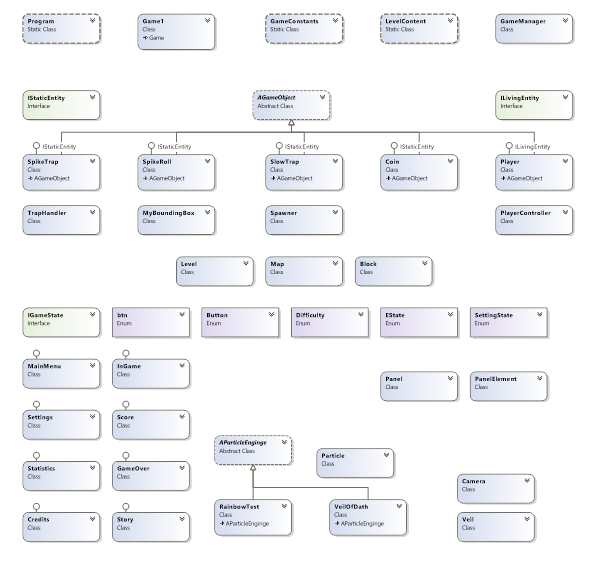
\includegraphics[width=1\textwidth]{classdiagramm.png}
	\caption{Klassendiagramm Veil of Death
		\label{fig:classdiagramm}}
\end{figure}

\newpage
\noindent Die Game-Klasse ist die Hauptklasse unseres Spieles. Von Ihr aus geht der allgemeine Game-Loop, der in allen Zuständen des Spiels vorkommt. Die unterschiedlichen Zustände des Spiels werden mit Hilfe eines Interfaces (IGameStates) mit gemeinsamen Funktionen (z.B. Initialisierung, Game-Loop, Draw) gespeist.
Für alle Objekte im Spiel die miteinander agieren können, haben wir eine übergeordnete abstrakte Klasse (AGameObject) erschaffen, von der die einzelnen Objektklassen erben.
Hierzu gibt es noch 2 verschiedene Interfaces, die die Objekte in starre (IStaticEntity) und bewegliche (IMovingEntity) einteilen.
Die Collision-Klasse berechnet alle Kollisionen des Spielers mit der Umgebung. Sie erhält Input
aus der Level- und Player-Klasse.
Die Player-Klasse, welche ebenfalls ein GameObject ist, wird durch die PlayerController-Klasse
gesteuert. Hier wird vor Allem die Bewegung des Spielers und die Kommunikation mit dem Rest der Umgebung (Position im Grid, Animation) übernommen.
Unsere Map-Klasse lädt die Spielwelt aus einer Bitmap-Grafik, welche die verschiedenen Blöcke kodiert.
Die Block-Klasse holt sich die Informationen, welches Model, oder Textur geladen werden soll aus einem Dictionary, die Klasse LevelContent.
Wir haben zwei zentrale Klassen für wichtige Steuerungs- und Speicherfunktionen. GameConstants ist eine statische Klasse, die sämtliche wichtigen Einstellungen und Standartwerte für das Spiel beinhaltet. Des weiteren haben wir einen Singelton-Klasse implementiert, die zwischen den verschiedenen Leveln und GameStates die wichtigsten Informationen überträgt und managed.
Ein Gesamtüberblick über alle unserer Klassen sind der \ref{fig:classdiagramm} zu entnehmen.

\newpage

\subsubsection{Use-Cases}

% 1. Use-Case Hauptmenü

\begin{figure}[H]
	\centering
	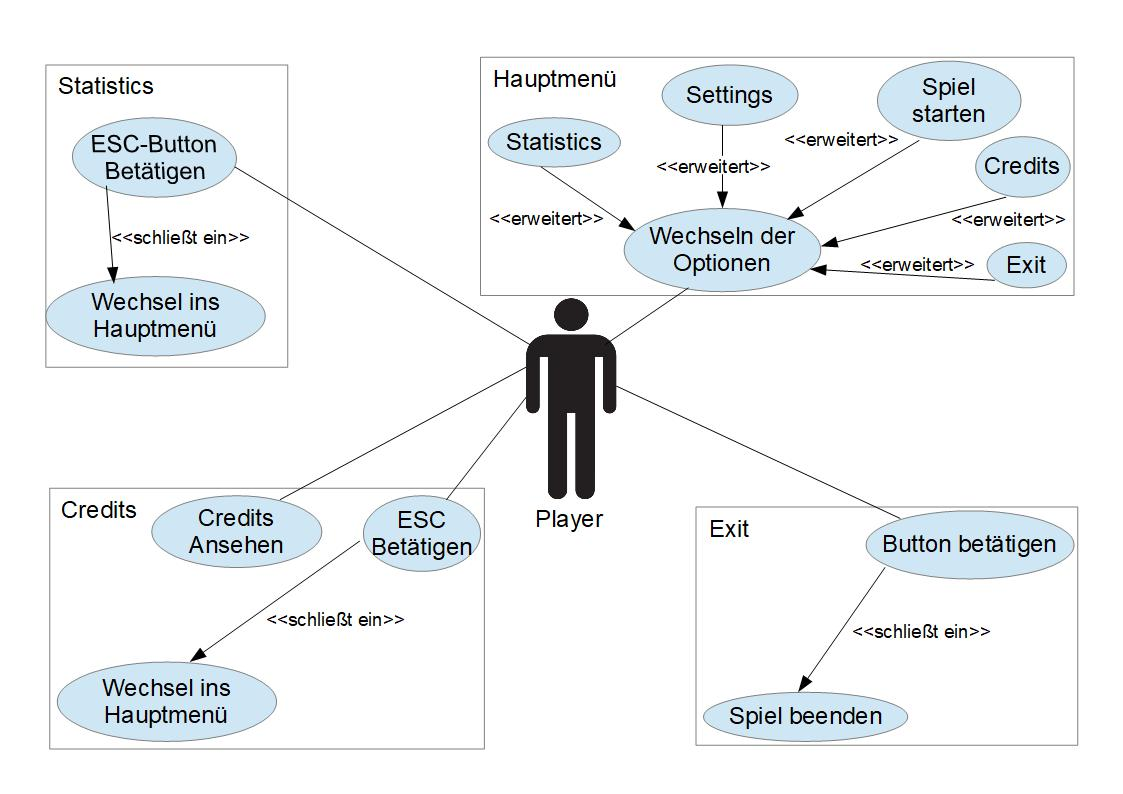
\includegraphics[width=1\textwidth]{UCM}
	\caption{Use-Case Hauptmenü 
		\label{fig:UCM}}
\end{figure}

Hauptmenü\newline
Das Hauptmenü zeigt eine Auswahl von fünf Buttons, die je nach Auswahl entsprechend hervorgehoben werden.
 Die Buttons sind:\newline
• Spiel starten\newline
Durch Spiel starten kommt man in den InGame Zustand des Spiels, in dem die einzelnen Level geladen und gestartet werden. \newline
• Settings \newline
Hier können vom Spieler verschiedene Einstellungen vorgenommen werden.
z.B. Schwierigkeitsgrad, Lautstärke \newline
• Statistics \newline
In den Statistiken werden alle aktuellen Fortschritte angezeigt \newline
• Credits \newline
In den Credits gibt es eine kurze Nennung der am Spiel beteiligten Teammitglieder, mit ihren jeweiligen Betätigungsfeldern \newline
• Exit\newline
Exit beendet das Programm. \newline

% 2. Use-Case Settings

\begin{figure}[H]
	\centering
	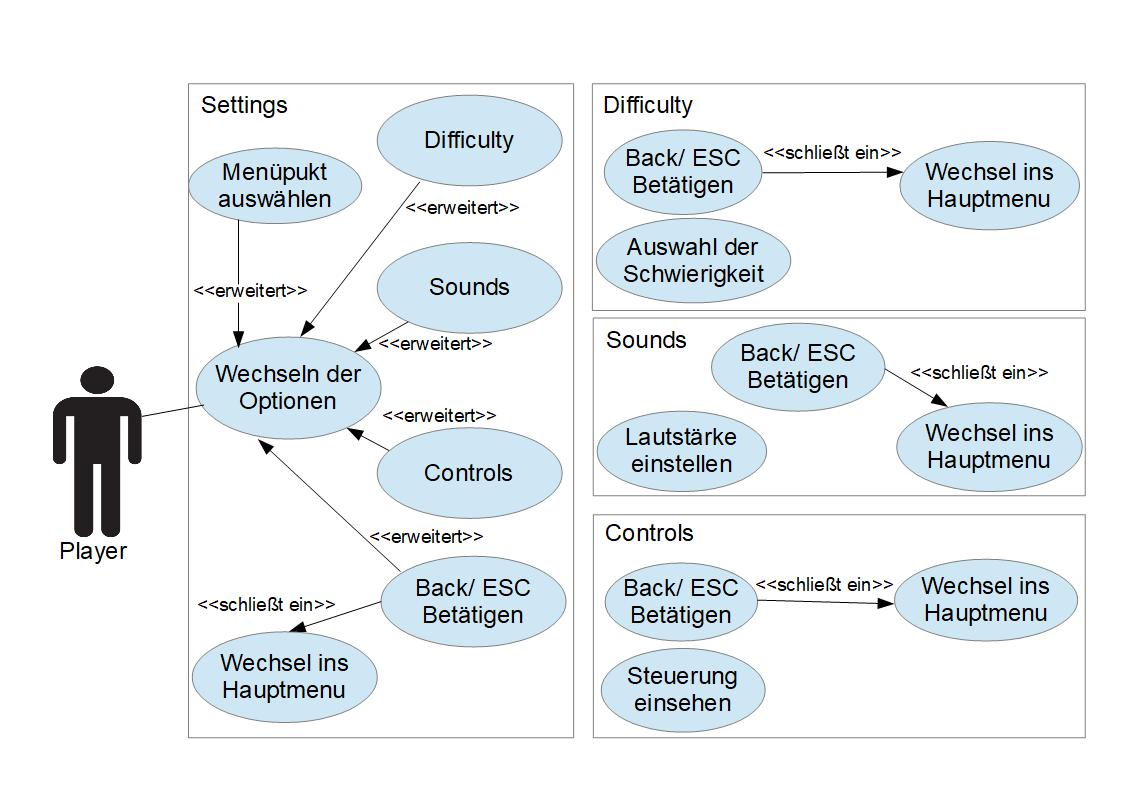
\includegraphics[width=1\textwidth]{UCS}
	\caption{Use-Case Settings
		\label{fig:UCS}}
\end{figure}

\noindent Settings\newline
In den Settings kann der Spieler die persönlichen Einstellungen an den folgenden Unterpunkten vornehmen.
Durch betätigen der Pfeiltasten oben/ unten kann der Spieler durch die Optionen wechseln. Mit der Enter-Taste wird
dann der Menüpunkt ausgewählt und der Spieler kann die Parameter an seine persönliche Belieben anpassen.
Folgende Optionen stehen zur Auswahl:\newline
• Difficulty\newline
In diesem Punkt der Spieler den Schwierigkeitsgrad des Spiels festlegen. Er hat die Auswahl zwischen den Optionen
easy, medium, hard, extreme.\newline
• Sounds\newline
Hier kann die Lautstärke des Spiels angepast werden.\newline
• Controls\newline
Unter diesem Punkt ist die Steuerung des Spiels sichtbar.\newline
\newline
Aus den jeweiligen Untermenüs kommt der Spieler mit dem Betätigen der ESC-Taste zurück zu den Einstellungsoptionen.
Mit einem weiteren Betätigen der ESC-Taste landet der Spieler wieder im Hauptmenü.\newline
\newline
Dieser Use-Case besteht im Grunde aus vier Separaten. Die Use-Cases auf der Rechten Seite erweitern jeweils die dazugehörigen
Optionen auf der linken Seite, dies können sie der \ref{fig:UCS} entnehmen. \newline


% 3. Use-Case Player - Environment

\begin{figure}[H]
	\centering
	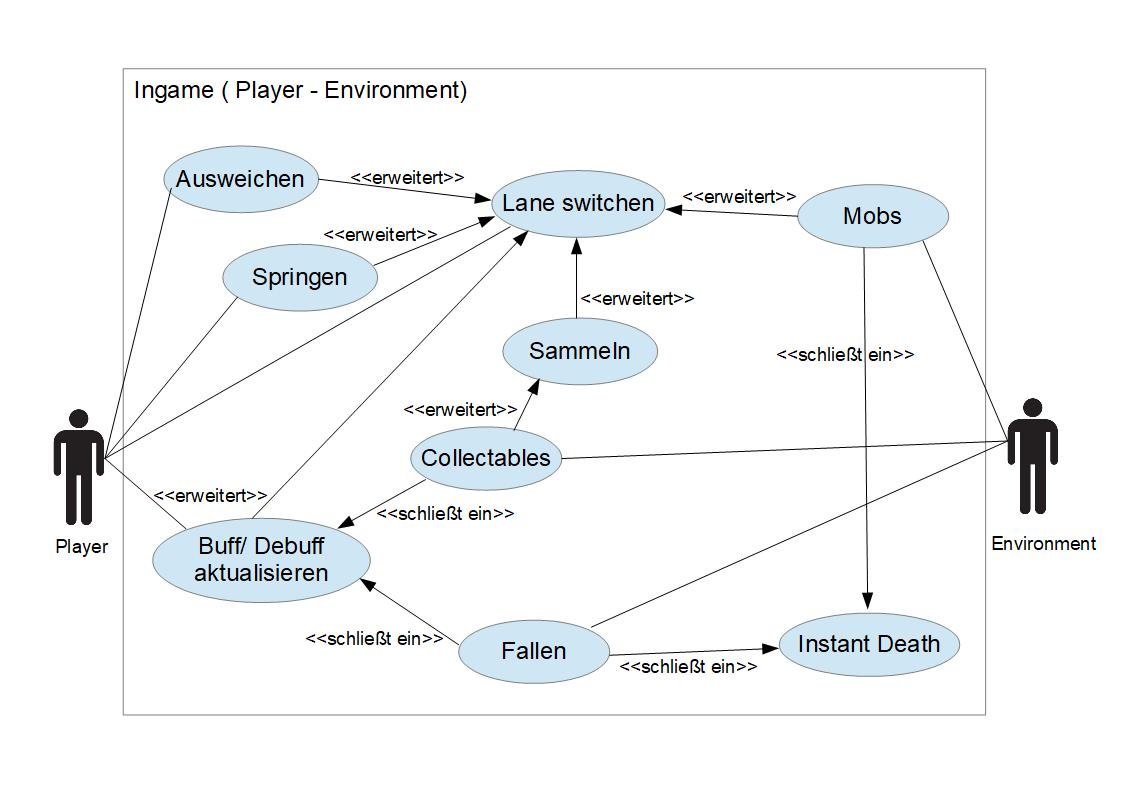
\includegraphics[width=1\textwidth]{UCIPE}
	\caption{Use-Case Ingame Player-Environment
		\label{fig:UCIPE}}
\end{figure}

\noindent Ingame (Player vs. Environment)\newline
Ingame kann der Spieler den Protagonisten verschiedene Aktionen ausführen lassen um
Hindernissen aus dem Weg zu gehen:\newline
• Lane wechseln\newline
• Springen\newline
• Dodgen\newline
Er kann verschiedene Collectables wie Coins oder Schwert aufnehmen, in dem er darüberläuft.
Er wechselt Lanes um Fallen, Hindernissen und Mobs aus dem Weg zu gehen, denn eine Kollision
bedeutet im besten Fall einen Debuff aber meist den sofortigen Tod. \newline


\subsection{Softwarearchitektur Entscheidungen}


Wir haben die Architektur der Software so gewählt, das wir die Struktur adaptiv halten. So halten wir uns die Möglichkeit offen, relativ einfach zusätzliche Komponenten in das Spiel zu integrieren.
Durch die Separierung des Codes in seine logischen Bereiche erhoffen wir uns, dass durch die Kapselung die Wartbarkeit und Lesbarkeit sich stark verbessert und auch Erweiterungen oder Änderungen an "fremden" Codestellen kein Problem darstellen.
\newline

\newpage
\section{Technische Mindestanforderungen}


Als Betriebssystem wird mindestens Windows 7 vorausgesetzt. Die Grafikkarte sollte mindestens DirectX10 und eine Auflösung von mindestens 1200*700 unterstützen. Es sollte sowohl eine
Soundkarte als auch eine Möglichkeit zur Soundausgabe in dem Gerät enthalten sein, da dies das Spielerlebnis deutlich verbessert.
Es ist möglich das Spiel mit einem Controller oder per Tastatur zuspielen.\newline

\vspace{1cm}
\section{Projektmanagement}


Github unterstützt inzwischen das Projektmanagement mit einer weiten Palette an Tools und UIs, sodass wir uns entschieden haben GitHub neben der Versionsverwaltung auch als zentrales Werkzeug für die Projektverwaltung zu benutzen.
Neben der Einteilung der verschiedenen Arbeitspakete in Meilensteine haben wir uns auch dazu entschlossen mit dem Kanban zu arbeiten. So hat jedes Teammitglied immer die aktuellen Status des Projektes vor Augen. Um den Informationsfluss des Kanbans noch zu verstärken haben wir Gebrauch von sogenannten Labels gemacht, die mit farblichen Markierungen den einzelnen Aufgabenpakete zusätzliche Attribute verleihen. So war es uns möglich auf den ersten Blick zu sehen, welcher Task gerade bearbeitet wird und wo es Probleme oder Rückfragen gibt. Auch Bugs und andere Fehler haben wir als Tasks erfasst und mit auffälligen Roten Labels markiert. Dies ermöglichte eine sehr nutzerfreundliche Arbeit an einer einzigen "Leinwand" 
Ein Momentaufnahme des Kanbans in der späteren Projektphase ist der \ref{fig:kanban} zu entnehmen.

\begin{figure}
	\centering
	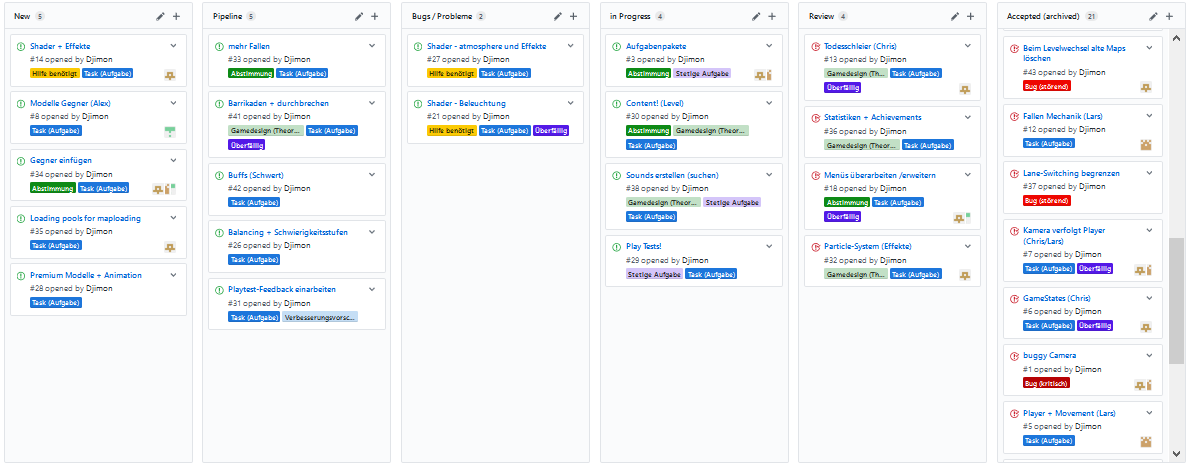
\includegraphics[width=1\textwidth]{kanban.png}
	\caption{Kanban (Anfang September 2017)
		\label{fig:kanban}}
\end{figure}

\newpage

\subsection{Meilensteinplanung - Arbeitspakete}


\subsubsection{Meilenstein 1: “technically it’s finished” (Deadline 04.05.)}
Game-Summary (Einleitung): Alex\newline
Coding Conventions: Chris\newline
Bibliotheken und Frameworks: Lars\newline
Verwendete Tools: Chris\newline
UML- und Klassendiagramme: Lars\newline
Projektmanagement, Aufgabenpakete: Chris\newline
Technische Mindestanforderung: Lars\newline
(Als Aufgaben nehmen wir jeweils die Überschriften und wer sie bearbeitet hat)\newline
\newline
\subsubsection{Meilenstein 2: “Welcome to the Core” (Deadline 31.05.)}
Gamestates: Chris\newline
Player: Lars\newline
Movement: Lars
MapGeneration (Bitmap): Chris\newline
StartMenü: Alex\newline
Modell Player: Alex\newline
Modelle Wände, Boden: Alex\newline
Texturen: Wände und Boden: Chris, Alex\newline
Model Collactables: Alex\newline
\newline
\subsubsection{Meilenstein 3: “Gimme some Feedback” (Deadline 30.06..)}
GUI + Scoresystem: Lars, Chris\newline
SoundSystem: Lars\newline
VisualEffects: Chris, Alex\newline
Prototyp Shader: Chris\newline
Fallen Mechaniken: Lars\newline
Mechanik des Todes Schleier: Chris\newline
Model Fallen: Alex\newline
Model Gegner: Alex\newline
Refactoring: Chris\newline
\subsubsection{Meilenstein 4: “Level 1 Completeted” (Deadline 31.07.)}
Ein Komplettes Level mit allen mechaniken Spielbar: Lars\newline
Prototyp Proceduale mapgeneration: Chris\newline
Animationen Laufen, Springen, Rutschen: Alex\newline
Weitere Shader für Effekte und Postprocessing: Chris\newline
Balancing Belohnung und Score: Lars\newline
Levelübersicht: Chris\newline
\subsubsection{Meilenstein 5: “This won’t work” (Deadline 31.08.)}
Level 2,3 (4,5): Lars\newline
Procedural Mapgeneration: Chris\newline
Playtests, Feedback: Alle\newline
Balancing Belohnung, Bestrafung: Lars\newline
Polishing Models und Animationen: Alex\newline
Polishing Menüs: Alex\newline
Achievements: Alle\newline
Refactoring: Lars, Chris\newline
\subsubsection{Meilenstein 6: “It lives!” (Deadline 19.09.)}
Debugging: Alle\newline
Polishing: Alle\newline
...\newline

	
\end{document}



